%Matteo Kumar - Leonard Schatt
% Fortgeschrittenes Physikalisches Praktikum

% Teilauswertung SE

\section{Spektrale Empfindlichkeit}
\subsection{Lock-in-Verstärker}
Um den Photostrom $I_{Ph}$ zu berechnen, muss zunächst die am Lock-in-Verstärker abgelesene Spannung in die tatsächlich anliegende Spannung umgerechnet werden. Der Verstärker hat als Output einen Wert zwischen $0$V und $10$V. Berücksichtigt man noch die Sensitivity des Verstärkers erhält man für die anliegende Spannung $U_{rms}$: \\

\begin{equation}
U_{rms} = \frac{U_{angezeigt}}{10V} \cdot Sensitivity
\end{equation}

Nun muss noch berücksichtigt werden, dass der Lock-in-Verstärker das Messsignal, das durch den Chopper (annähernd) reckteckförmig moduliert wurde, mit dem sinusförmigen Referenzsignal des Choppers faltet, bevor die Faltung durch einen Tiefpass geleitet wird. Ein Rechtecksignal kann geschrieben werden als:\\

\begin{equation}
f_{Rechteck} = \frac{4U_{Rechteck}}{\pi} \sum_{k=1}^\infty \frac{sin((2k-1)\omega t)}{2k-1}  ,
\end{equation}

wobei $U_{Rechteck}$ die Amplitude des Signals bezeichnet.
Faltet man dieses nun mit einem Signal der Frequenz $\omega$, so trägt nach durchlaufen des Tiefpasses nur der Anteil am Rechtecksignal mit ebenfalls $\omega$ bei, also der Term für $k = 1$. Die gemessene Spannung ergibt sich also zu: \\

\begin{align}
U_{ein} &= \frac{4U_{Rechteck}}{\pi} sin(\omega t) \nonumber \\ 
\implies U_{rms} &= \frac{1}{\sqrt{2}} \frac{4U_{Rechteck}}{\pi}
\end{align}

Stellt man nun nach der Amplitude der Spannung $U_{Rechteck}$ um, so erhält man:

\begin{align}
U_{Rechteck} &= \frac{\pi \sqrt{2}}{4} U_{rms} \\
\implies U_{Rechteck} &= \frac{\pi \sqrt{2}}{4} \cdot Sensitivity \cdot \frac{U_{angezeigt}}{10V}
\end{align}

Um den Photostrom $I_{Ph}$ zu erhalten, muss jetzt nur noch die tatsächliche Spannung mithilfe des Faktors des U/I-Verstärkers umgerechnet werden. 
Dabei muss noch ein Faktor 2 berücksichtigt werden, da der Chopper die Hälfte des einfallenden Lichts abhält:\\

\begin{align}
I_{Ph} &= \frac{2U_{Rechteck}}{1 \frac{kV}{A}} \nonumber \\
 &= \frac{\pi \sqrt{2}}{4} \cdot Sensitivity \cdot \frac{U_{angezeigt}}{10000 \frac{V^2}{A}}
\label{eq:IPh}
\end{align}


\subsection{Spektrale Empfindlichkeit SR und Externe Quanteneffizienz EQE}

Die Spekrtale Empfindlichkeit $SR$ berechnet sich nach:
\begin{equation}
SR = \frac{I_{Ph}}{P_\lambda},
\end{equation}

mit Photostrom $I_{Ph}$ aus Gl. \ref{eq:IPh}. Dabei muss noch berücksichtigt werden, dass für alle Messwerte noch der Photostrom aus der
Untergrundsmessung abgezogen wird. \\
Die in die Zelle einfallende Leistung $P_{\lambda}$ muss erst noch aus der in das Powermeter einfallende Leistung berechnet werden. Es gilt:
\begin{align}
P_{PM} &= P_{ges} R \nonumber \\
P_{\lambda} &= P_{ges} T \nonumber \\
\implies P_{\lambda} &= P_{PM} \frac{T}{R},
\end{align}

mit Reflektionskoeffizient des Strahlteilers $R$, Transmissionskoeffizient $T$ und gesamter Lichtleistung vor Auftreffen auf den Teiler $P_{ges}$.
Für die Werte von $\frac{T}{R}$ wurden die Inversen von Abschätzungen der Werte $\frac{R}{T}$ aus Anhang $A.2$ des Versuchsskriptes benutzt. Bei der 
Berechnung der einfallenden Leistung muss für das CIS-Modul noch ein Faktor $\frac{1}{11}$ berücksichtigt werden, da das Modul aus 11 
einzelnen Zellen besteht und die Leistung sich demnach auf diese näherungsweise gleichmäßig aufteilt (tatsächlich wohl eher ungleichmäßig, 
je nach Positionierung der Zelle im Strahl, dennoch soll dies zur Vereinfachung der Rechnung angenommen werden). Der Photostrom bleibt 
allerdings gleich dem gemessenen, da die Zellen in Reihe geschalten sind.

Aus den Werten für $SR$ lassen sich nun auch die für die Externe Quanteneffizienz $EQE$ berechnen:
\begin{align}
EQE &= \frac{hc}{e} \frac{SR}{\lambda}
\label{eq:eqe}
\end{align}

Die berechneten Werte finden sich in Tab. \ref{tab:32mono} - \ref{tab:32cis} wieder. Die Messdaten können dem Protokoll entnommen werden.
\\

\begin{center}
%\captionof{table}{Berechnete Werte für die monokristalline Siliziumzelle}
\begin{tabular}{rrrrrr}
    $Wellenlänge (nm)$ &  $I_{Ph} (A)$ &    $\frac{T}{R}$ &  $P_{ges} (\mu W)$ &  $SE (\frac{A}{W})$ &       $EQE$ \\
    \hline
    363.2 &  0.000004 &  1.2262 &   57.8540 &  0.0682 &  0.2330 \\
    400.3 &  0.000013 &  1.2239 &   88.2741 &  0.1521 &   0.4713 \\
    450.8 &  0.000037 &  1.2254 &  150.8578 &  0.2445 &  0.6725 \\
    499.2 &  0.000056 &  1.2004 &  183.5534 &  0.3059 &  0.7597 \\
    599.1 &  0.000099 &  1.1806 &  249.8229 &  0.3959 &    0.8194 \\
    699.9 &  0.000113 &  1.1587 &  229.3163 &  0.4914 &  0.8705 \\
    799.5 &  0.000103 &  1.1876 &  179.2161 &  0.5754 &   0.8924 \\
    899.8 &  0.000156 &  1.1402 &  244.3557 &  0.6393 &  0.8809 \\
    949.4 &  0.000166 &  1.0604 &  245.0689 &  0.6773 &  0.8845 \\
    1000.5 &  0.000162 &  1.0438 &  250.4175 &  0.6460 &  0.8005 \\
    1051.2 &  0.000086 &  1.0373 &  177.9045 &  0.4823 &  0.5688 \\
    1099.6 &  0.000021 &  1.0395 &   84.6465 &  0.2434 &  0.2745 \\
    1123.3 &  0.000013 &  1.0411 &   83.7376 &  0.1553 &  0.1715 \\
    
\end{tabular}
\captionof{table}{Berechnete Werte für die monokristalline Siliziumzelle}
\label{tab:32mono}
\end{center}

\begin{center}
\begin{tabular}{rrrrrr}
    $Wellenlänge (nm)$ &  $I_{Ph} (A)$ &    $\frac{T}{R}$ &  $P_{ges} (\mu W)$ &  $SE (\frac{A}{W})$ &       $EQE$ \\
    \hline
    363.2 &  0.000003 &  1.2262 &   55.2053 &  0.0492 &   0.1680 \\
    400.3 &  0.000010 &  1.2239 &   84.1738 &  0.1199 &   0.3714 \\
    450.8 &  0.000031 &  1.2254 &  143.6274 &  0.2141 &   0.5889 \\
    499.2 &  0.000052 &  1.2004 &  174.9099 &  0.2982 &   0.7407 \\
    599.1 &  0.000090 &  1.1806 &  237.7804 &  0.3772 &   0.7807 \\
    699.9 &  0.000100 &  1.1587 &  217.1494 &  0.4622 &    0.8188 \\
    799.5 &  0.000088 &  1.1876 &  168.8836 &  0.5193 &   0.8054 \\
    899.8 &  0.000111 &  1.1402 &  210.7183 &  0.5280 &   0.7275 \\
    949.4 &  0.000109 &  1.0604 &  213.9978 &  0.5074 &   0.6626 \\
    1000.5 &  0.000110 &  1.0438 &  261.7954 &  0.4207 &   0.5213 \\
    1051.2 &  0.000042 &  1.0373 &  179.9792 &  0.2308 &   0.2722 \\
    1099.6 &  0.000008 &  1.0395 &   85.8004 &  0.0876 &  0.09879 \\
    1123.3 &  0.000004 &  1.0411 &   84.3831 &  0.0461 &  0.05088 \\

\end{tabular}
\captionof{table}{Berechnete Werte für die multikristalline Siliziumzelle}
\label{tab:32multi}
\end{center}

\begin{center}
\begin{tabular}{rrrrrr}
    $Wellenlänge (nm)$ &  $I_{Ph} (A)$ &    $\frac{T}{R}$ &  $P_{ges} (\mu W)$ &  $SE (\frac{A}{W})$ &       $EQE$ \\
    \hline
    363.2 &  6.1089e-08 &  1.2262 &    4.9607 &  0.01231 &  0.04203 \\
    400.3 &  8.5614e-07 &  1.2239 &    7.5865 &  0.1128 &   0.3495 \\
    450.8 &  3.0420e-06 &  1.2254 &   13.0013 &  0.2339 &   0.6435 \\
    499.2 &  4.5348e-06 &  1.2004 &   15.8245 &  0.2865 &   0.7117 \\
    599.1 &  8.1713e-06 &  1.1806 &   21.5734 &  0.3787 &   0.7838 \\
    699.9 &  9.0599e-06 &  1.1587 &   19.8567 &  0.4562 &   0.8082 \\
    799.5 &  8.1047e-06 &  1.1876 &   15.5581 &  0.5209 &   0.8078 \\
    899.8 &  1.1148e-05 &  1.1402 &   20.4312 &  0.5456 &   0.7518 \\
    949.4 &  1.1281e-05 &  1.0604 &   20.3412 &  0.5546 &   0.7242 \\
    1000.5 &  1.2347e-05 &  1.0438 &   23.4484 &  0.5265 &   0.6525 \\
    1051.2 &  7.5271e-06 &  1.0373 &   16.3334 &  0.4608 &   0.5435 \\
    1099.6 &  2.6954e-06 &  1.0395 &    7.7783 &  0.3465 &   0.3907 \\
    1123.3 &  2.1823e-06 &  1.0411 &    7.6569 &  0.2850 &   0.3145 \\

\end{tabular}
\captionof{table}{Berechnete Werte für das CIS-Modul}
\label{tab:32cis}
\end{center}

Die Lage der Bandkanten sind für Silizium $1,1242$eV 
(\url{https://www.pveducation.org/pvcdrom/materials/general-properties-of-silicon}, Stand: 9.9.21) und für CIS $1,02$eV 
(\url{https://www.pveducation.org/pvcdrom/materials/cuinse2}, Stand: 9.9.21). Die Lage dieser im Wellenängenraum berechnet sich nach: \\

\begin{align}
\lambda_{Bandkante} &= \frac{hc}{E_{Bandkante}}
\end{align}

Daraus folgt: \\

\begin{equation}
\lambda_{Si} = 1102,866 nm, \qquad \lambda_{CIS} = 1215,531 nm
\label{eq:bandkante}
\end{equation}

In den folgenden Abbildungen \ref{bild:SRall} und \ref{bild:allEQE} wurden die spektrale Empfindlichkeit und die externe 
Quanteneffizienz gegen die Wellenlänge aufgetragen.
Dabei wurden auch die jeweiligen Bandkanten aus Gl. \ref{eq:bandkante} eingezeichnet.

\begin{figure}[h]
    \centering
    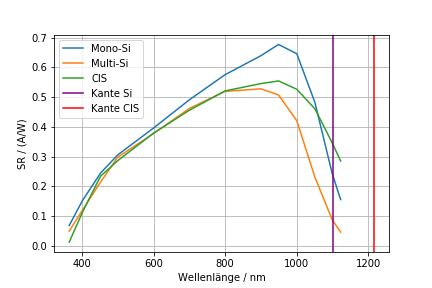
\includegraphics[scale=0.75]{Bilder/32allSRverb.png}
    \caption{Verlauf der gemessenen Werte von $SR$ der verschiedenen Zellen aufgetragen gegen die Wellenlänge}
    \label{bild:SRall}
\end{figure}


\begin{figure}[ht]
    \centering
    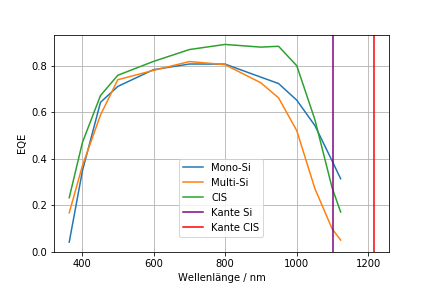
\includegraphics[scale=0.75]{Bilder/32allEQEverb.png}
    \caption{Verlauf der gemessenen Werte von $EQE$ der verschiededen Zellen aufgetragen gegen die Wellenlänge}
    \label{bild:allEQE}
\end{figure}

\clearpage

Bei den Siliziummodulen ist zu erkennen, dass sich trotz 
Überschreitung der Bandkante dennoch eine endliche spektrale Empfindlichkeit aus den Messungen ergibt. 
%Dies ist auch nicht alleine durch die Driftleistung des Powermeters zu erklären, da diese im Nanowatt-Bereich liegen. 
Die Bandkante des CIS-Moduls liegt bei einer höheren Wellenlänge als der Messpunkt der größten Wellenlänge, deshalb kann nicht mit 
Sicherheit gesagt werden, ob das Problem des Überschreitens der Bandkante hier auch auftreten würde. Dennoch lässt sich an Abb. 
\ref{bild:SRall} gut erkennen, dass die Lage der Bandkante annäherungsweise mit dem Nulldurchgang des Graphen der spektralen Empfindlichkeit
übereinstimmt. Als Erklärung, dass hinter der Bandkante noch Messwerte vorliegen, können Messfehler dienen. Allerdings ist die 
Überschreitung nicht sehr groß, daher kann auch eine Abweichung der realen Solarzelle vom Bändermodell die Ursache sein. \\


Als Anhaltspunkt zum Vergleich sollen die Abb. \ref{bild:ThSR} und \ref{bild:ThEQE} dienen, in denen $SR$ und $EQE$ für eine multikristalline Solarzelle 
gegen die Wellenlänge aufgetragen ist. Es ist gut zu erkennen, dass die Form des Verlaufs mit den gemessenen Kurven übereinstimmt. Im 
Vergleichsgraphen werden zwar deutlich höhere Werte für $SR$ und $EQE$ erreicht, es ist aber anzunehmen, dass der Idealitätsfaktor $n$ 
der dort in präzisen Labormessungen verwendeten Zellen deutlich besser war und dass infolgedessen die Ausbeute höher war.
Aber auch in diesen Messungen ist deutlich zu sehen, dass die Bandkante bei $\lambda = 1102,866 nm$ deutlich überschritten wird. Somit
kann das Überschreiten in unserer Messung wahrscheinlich auf die Abweichungen der realen Zelle im Bändermodell zurückgeführt werden.

\begin{figure}[ht]
    \centering
    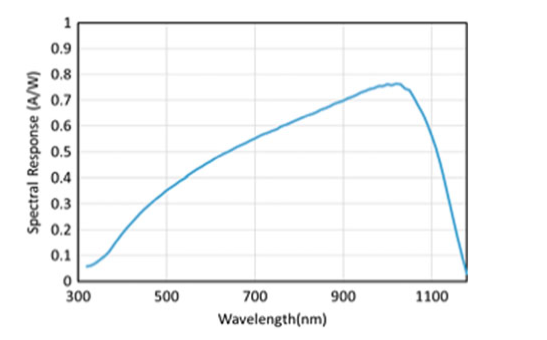
\includegraphics[scale=0.75]{Bilder/TheorieSR.png}
    \caption{Vergleichsdaten für den Verlauf von $SR$ einer multikristallinen Siliziumzelle \protect \footnotemark}
    \label{bild:ThSR}
\end{figure}

\footnotetext{\cite{Shah2020}, S.68}

\begin{figure}[ht]
    \centering
    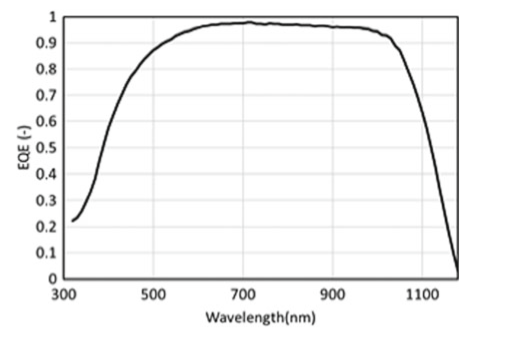
\includegraphics[scale=0.75]{Bilder/TheorieEQE.png}
    \caption{Vergleichsdaten für den Verlauf von $EQE$ einer multikristallinen Siliziumzelle \protect \footnotemark}
    \label{bild:ThEQE}
\end{figure}

\footnotetext{\cite{Shah2020}, S.68}



\subsection{Ideale Externe Quanteneffizienz}

Nimmt man nun eine ideale externe Quanteneffizienz von $1$ an, folgt aus Gl. \ref{eq:eqe}:
\begin{align}
SR &= \frac{e}{hc}\lambda
\end{align}

Der Graph der spektralen Empfindlichkeit ist somit zunächst eine Gerade mit Steigung $\frac{e}{hc}$, bis diese Gerade auf die
Vertikale der bandkante trifft. Da nach Überschreitung der Bandkante kein Stromfluss mehr möglich ist (höhere Wellenlänge 
$\leftrightarrow$ niedrigere Energie), fällt die Gerade dort abrupt ab. Der Verlauf ist in Abb. \ref{bild:idealEQEverb} zu sehen.
Hierbei ist der Verlauf beider Modularten erst die rote Ursprungsgerade, die dann im Fall der Siliziumzellen mit der violetten
Vertikalen, im Fall des CIS-Moduls mit der roten Vertikalen abfallen.
Betrachtet man die Graphen der Messwerte wird klar, dass die verwendeten Zellen zwar kein Ideal sind. Dennoch lässt sich in 
ihrem Verlauf ein Trend zum idealen Graphen erkennen. Dieser Umstand soll in der
nächsten Teilaufgabe weiter vertieft werden, wenn der Idealitätsfaktor bestimmt wird.

\begin{figure}[ht]
    \centering
    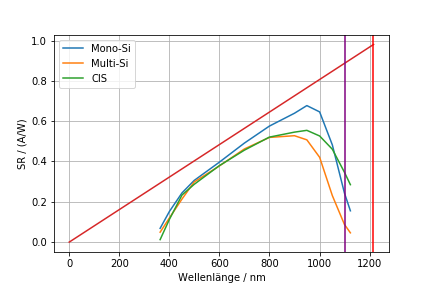
\includegraphics[scale=0.75]{Bilder/32idealEQEverb.png}
    \caption{Verlauf von $SR$ bei einer idealen $EQE = 1$; der Graph für die Si-Zellen fällt mit der violetten Vertikalen ab, der für
    das CIS-Modul mit der roten. Zum Vergleich die Messwerte für $SR$.}
    \label{bild:idealEQEverb}
\end{figure}
 
\newpage